\subsection{Active Shunt-Shunt Feedback (ASSFB) CTLE}
\label{sec:assfb_ctle}

The Active Shunt-Shunt Feedback (ASSFB) CTLE enhances bandwidth and peaking performance by applying negative feedback around a conventional SD-CTLE stage. This architecture extends poles outward through impedance reduction at both input and output nodes, enabling higher peaking frequencies and improved equalization capabilities for severe channel losses exceeding 25 dB at the Nyquist frequency.

\subsubsection*{Circuit Architecture and Operation}
\label{subsec:assfb_architecture}

\begin{figure}[H]
    \centering
    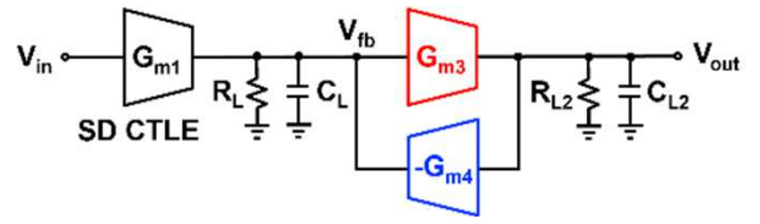
\includegraphics[width=0.9\textwidth]{img/CTLE_img/assfb_block diagram.png}
    \caption{Block diagram representation of the active shunt-shunt feedback system.}
    \label{fig:assfb_block_diagram}
\end{figure}

The ASSFB-CTLE concept, illustrated in Figure~\ref{fig:assfb_block_diagram}, builds upon a conventional SD-CTLE ($G_{m1}$, $R_L$, $R_s$, $C_s$) by adding two feedback transconductance stages: $G_{m3}$ (sensing) and $G_{m4}$ (mixing). The feedback path senses the output voltage through $G_{m3}$ and injects a compensating current at the input via $G_{m4}$, creating a shunt-shunt configuration. This feedback mechanism reduces both input and output impedances by a factor of $(1 + A\beta)$, where $A\beta = G_{m3}G_{m4}R_LR_{L2}$ is the loop gain. The impedance reduction enables pole pushing to higher frequencies, extending the bandwidth beyond conventional SD-CTLE limitations.

\begin{figure}[H]
    \centering
    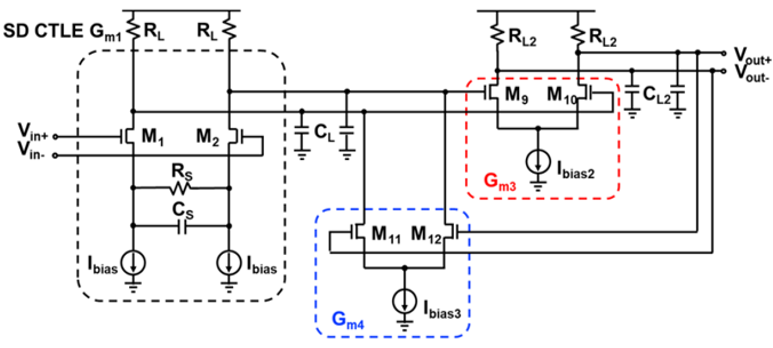
\includegraphics[width=0.8\textwidth]{img/CTLE_img/assfb_schematic.png}
    \caption{Active shunt-shunt feedback CTLE circuit implementation with feedback transconductance stages [H. Hsu TCAS I '25].}
    \label{fig:assfb_schematic}
\end{figure}

The circuit implementation, shown in Figure~\ref{fig:assfb_schematic}, realizes the block diagram concept with specific transistor-level design. The main SD-CTLE consists of $M_1$-$M_2$ with degeneration $R_s$-$C_s$, while the feedback network is implemented through transistors $M_9$-$M_{10}$ ($G_{m3}$) and $M_{11}$-$M_{12}$ ($G_{m4}$). The shunt-shunt configuration effectively reduces impedances at both input and output nodes, with the loop gain $A\beta$ controlling the degree of pole pushing and bandwidth extension.

\subsubsection*{Frequency Response Analysis}
\label{subsec:assfb_freq_response}

\begin{figure}[H]
    \centering
    \begin{minipage}{0.48\textwidth}
        \centering
        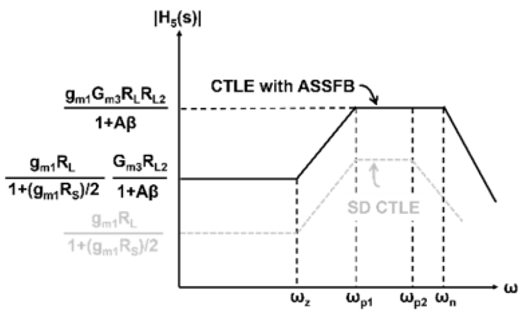
\includegraphics[width=0.95\textwidth]{img/CTLE_img/assfb_assym.png}
        \caption{Asymptotic frequency response comparison.}
        \label{fig:assfb_assym}
    \end{minipage}
    \hfill
    \begin{minipage}{0.48\textwidth}
        \centering
        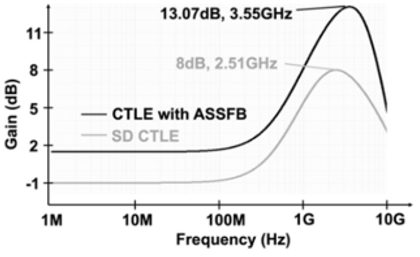
\includegraphics[width=0.95\textwidth]{img/CTLE_img/assfb_real.png}
        \caption{Actual response in 180nm technology.}
        \label{fig:assfb_real}
    \end{minipage}
\end{figure}

The transfer function for the ASSFB-CTLE is:

\[
H_5(s) = \frac{g_{m1} R_L}{1 + \frac{g_{m1}R_s}{2}} \cdot \frac{G_{m3} R_{L2}}{1 + A\beta} \cdot \frac{1 + \frac{s}{\omega_z}}{1 + \frac{s}{\omega_{p1}}} \cdot \frac{1}{1 + \frac{2\zeta_3}{\omega_{n3}} s + \frac{s^2}{\omega_{n3}^2}}
\]

where the key frequency parameters are:

\[
\begin{aligned}
\omega_{n3} &= \sqrt{\frac{1 + A\beta}{R_L C_L R_{L2} C_{L2}}}, &\quad
\zeta_3 &= \frac{\omega_{n3}}{2} \cdot \frac{R_L C_L R_{L2} C_{L2}}{1 + A\beta}, &\quad
A\beta &= G_{m3}G_{m4}R_LR_{L2}
\end{aligned}
\]

As shown in Figure~\ref{fig:assfb_real}, the ASSFB-CTLE achieves 13.07 dB peaking at 3.55 GHz compared to SD-CTLE's 8 dB at 2.51 GHz, representing a 63.4\% improvement in peaking gain and 41.4\% increase in peaking frequency.

\subsubsection*{Design Knobs and Tunability}
\label{subsec:assfb_design_knobs}

\subsubsection*{Effect of Transistor Width $W_{11,12}$}
\label{subsubsec:effect_w1112}

\begin{figure}[H]
    \centering
    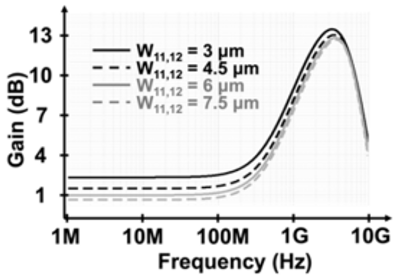
\includegraphics[width=0.4\textwidth]{img/CTLE_img/assfb_effect of w.png}
    \caption{Frequency response variation with increasing $W_{11,12}$ in 180nm technology.}
    \label{fig:assfb_effect_w}
\end{figure}

The transistor widths $W_{11,12}$ control $G_{m4} = g_{m11,12}$, which directly affects the loop gain $A\beta = G_{m3}G_{m4}R_LR_{L2}$. As shown in Figure~\ref{fig:assfb_effect_w}:

\begin{itemize}
    \item Increasing $W_{11,12}$ from 3 µm to 7.5 µm enhances peaking gain by approximately 2 dB.
    \item Larger $W_{11,12}$ increases $A\beta$, extending $\omega_{n3}$ to higher frequencies.
    \item However, increased $A\beta$ reduces $\zeta_3$, requiring careful stability design.
\end{itemize}

\subsubsection*{Effect of Bias Current $I_{\text{bias3}}$}
\label{subsubsec:effect_ibias3}

\begin{figure}[H]
    \centering
    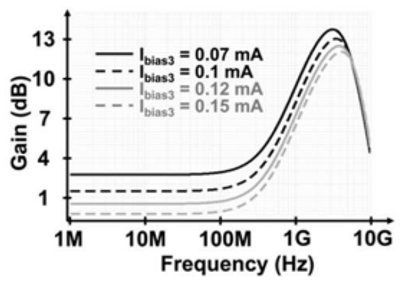
\includegraphics[width=0.4\textwidth]{img/CTLE_img/assfb_effect of i bias.png}
    \caption{Frequency response variation with increasing $I_{\text{bias3}}$ in 180nm technology.}
    \label{fig:assfb_effect_ibias}
\end{figure}

The bias current $I_{\text{bias3}}$ sets $G_{m4}$ transconductance, providing dynamic control over feedback strength. As shown in Figure~\ref{fig:assfb_effect_ibias}:

\begin{itemize}
    \item Higher $I_{\text{bias3}}$ increases $G_{m4}$, boosting $A\beta$ and extending bandwidth.
    \item Power consumption increases linearly with $I_{\text{bias3}}$, creating a power-performance trade-off.
\end{itemize}

The design expressions affected by these parameters are:

\[
\begin{aligned}
\text{DC Gain} &= \frac{g_{m1}R_L}{1 + \frac{g_{m1}R_s}{2}} \cdot \frac{G_{m3}R_{L2}}{1 + A\beta}, &\quad
\text{Peaking Gain} &= g_{m1}R_L \cdot \frac{G_{m3}R_{L2}}{1 + A\beta}, &\quad
A\beta &= G_{m3}G_{m4}R_LR_{L2}
\end{aligned}
\]

\subsubsection*{Design Trade-offs and Guidelines}
\label{subsec:assfb_tradeoffs}

\begin{table}[H]
\centering
\label{tab:assfb_tradeoffs}
\begin{tabular}{ >{\raggedright\arraybackslash}p{0.13\textwidth} 
                 >{\raggedright\arraybackslash}p{0.30\textwidth} 
                 >{\raggedright\arraybackslash}p{0.25\textwidth} 
                 >{\raggedright\arraybackslash}p{0.3\textwidth} }
\toprule
\textbf{Parameter} & \textbf{Benefit} & \textbf{Risk} & \textbf{Design Guideline} \\
\midrule
$W_{11,12}$ & Increases $A\beta$, higher $\omega_{n3}$ & Reduces $\zeta_3$, stability risk & Size for $\zeta_3 > 0.7$ \\
\midrule
$I_{\text{bias3}}$ & Tunable $G_{m4}$, adaptive peaking & Power consumption, thermal noise & Adaptive bias for PVT \\
\midrule
$A\beta$ & Extends bandwidth, higher peaking freq & Complex stability analysis & Optimize for target $\omega_{n3}$ \\
\midrule
$\zeta_3$ & Ensures stability, controls ringing & Limits peaking if too high & Target $0.7 < \zeta_3 < 1.0$ \\
\midrule
Feedback & Pole pushing, bandwidth extension & Higher area and power & Use for severe loss channels \\
\bottomrule
\end{tabular}
\end{table}